\subsection{Chiến lược Cân bằng Dữ liệu (Resampling Comparative Analysis)}
\label{sec:5_3}

Dữ liệu chất lượng cao là nền tảng cốt lõi định đoạt sự thành bại của mọi mô hình Học máy. Tuy nhiên, đối với bài toán giao thông không gian - thời gian, việc sở hữu một bộ dữ liệu lớn không đồng nghĩa với việc sở hữu một bộ dữ liệu tốt. Mục này trình bày các thách thức về mặt phân phối dữ liệu và biện luận cho chiến lược "Cân bằng Lai" (Hybrid Resampling) mà đồ án đã thiết kế.

\subsubsection{Thách thức từ dữ liệu mất cân bằng cực hạn (Extreme Imbalance)}

\paragraph{a. Bản chất vật lý của sự mất cân bằng} \mbox{} \\
Trong các hệ thống AI ứng dụng vào thế giới thực, sự phân phối của dữ liệu hiếm khi đạt trạng thái đồng đều lý tưởng. Thống kê từ tập dữ liệu lịch sử thu thập trên mạng lưới giao thông cho thấy một hiện tượng Mất cân bằng cực hạn (Extreme Imbalance). Cụ thể, các trạng thái lưu thông từ Thông thoáng đến Ổn định (Lớp 0, 1, 2) chiếm tỷ trọng áp đảo lên tới hơn $90\%$. Ngược lại, các sự kiện ùn tắc nghiêm trọng (Lớp 4) và "Vỡ trận/Kẹt cứng" (Lớp 5) là những điểm dị thường (Anomalies), chỉ chiếm tỷ lệ vô cùng nhỏ nhoi, chưa tới $0.1\%$ trên tổng dung lượng dữ liệu.

Sự chênh lệch này không phải là lỗi hệ thống cảm biến, mà là phản ánh chính xác quy luật vật lý và hành vi xã hội: Giao thông đô thị phần lớn thời gian trong ngày duy trì ở trạng thái dòng tự do (free-flow) và chỉ sụp đổ cấu trúc vào một số khung giờ cao điểm hoặc khi có sự cố bất ngờ.

\paragraph{b. Bẫy "Nghịch lý độ chính xác" và Thiên kiến lớp đa số (Majority Class Bias)} \mbox{} \\
Dù hợp lý về mặt vật lý, sự mất cân bằng cực hạn này lại là một "bản án tử" đối với thuật toán tối ưu hóa của mạng nơ-ron nếu được đưa trực tiếp vào huấn luyện. Khi sử dụng dữ liệu thô, mô hình sẽ đối mặt với \textbf{Nghịch lý độ chính xác (Accuracy Paradox)}. Nếu một mạng Nơ-ron học cách gian lận bằng việc luôn luôn dự báo là "Thông thoáng" (Lớp 1) bất chấp dữ liệu đầu vào là gì, nó nghiễm nhiên đạt độ chính xác (Accuracy) tổng thể trên $90\%$. Thuật toán Gradient Descent sẽ ghi nhận đây là một chiến lược "thành công" để giảm thiểu hàm mất mát (Loss function) nhanh nhất. Hệ quả là, mô hình bị rơi vào bẫy Thiên kiến lớp đa số (Majority Class Bias), trở nên hoàn toàn "mù màu" và phớt lờ các tín hiệu của lớp thảm họa (Recall của Lớp 4, 5 tiệm cận $0\%$).

\paragraph{c. Tác động tiêu cực đến Đặc vụ Học tăng cường (DQN Agent)} \mbox{} \\
Đối với mạng Double DQN được thiết kế trong đồ án, sự mất cân bằng này còn gây ra hậu quả tàn khốc hơn ở khâu lấy mẫu kinh nghiệm (Experience Replay).

Bộ nhớ Replay Buffer lưu trữ các quá trình chuyển trạng thái (transitions). Nếu nạp dữ liệu thô, $99\%$ không gian trong Buffer sẽ chứa các mẩu kinh nghiệm nhàm chán của Lớp 0 và 1. Khi Agent bốc ngẫu nhiên một mẻ dữ liệu (Batch) để huấn luyện, xác suất bốc trúng một kinh nghiệm về "sự cố kẹt xe Lớp 5" là cực kỳ thấp. Thiếu đi sự "cọ xát" với các trạng thái nguy hiểm, Agent sẽ hình thành một chính sách (Policy) lười biếng, phản ứng chậm trễ và không thể kích hoạt kịp thời cảnh báo khi kẹt xe thực sự bắt đầu lan rộng.

Do đó, việc tái định hình lại không gian phân phối dữ liệu (Resampling) trước khi đưa vào huấn luyện không chỉ là một thủ thuật tiền xử lý, mà là một yêu cầu sinh tử để mô hình có thể phát hiện thảm họa.

\begin{figure}[H]
    \centering
    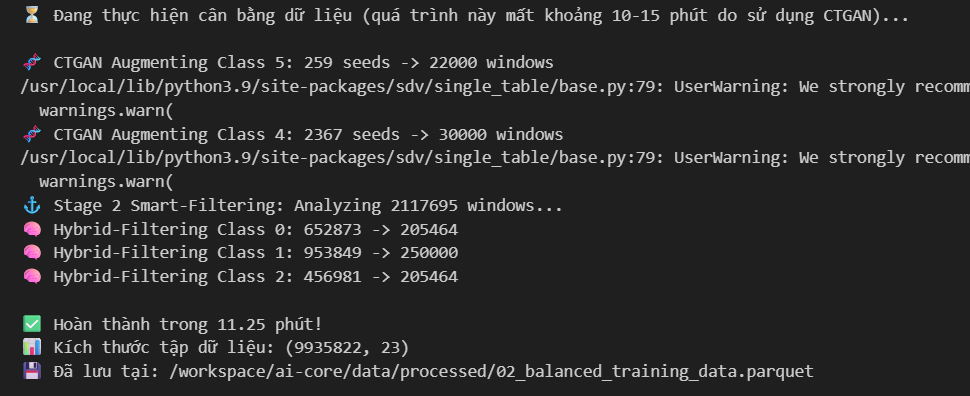
\includegraphics[width=0.8\textwidth]{Images/CH5/11b.png} \\
    \vspace{10pt}
    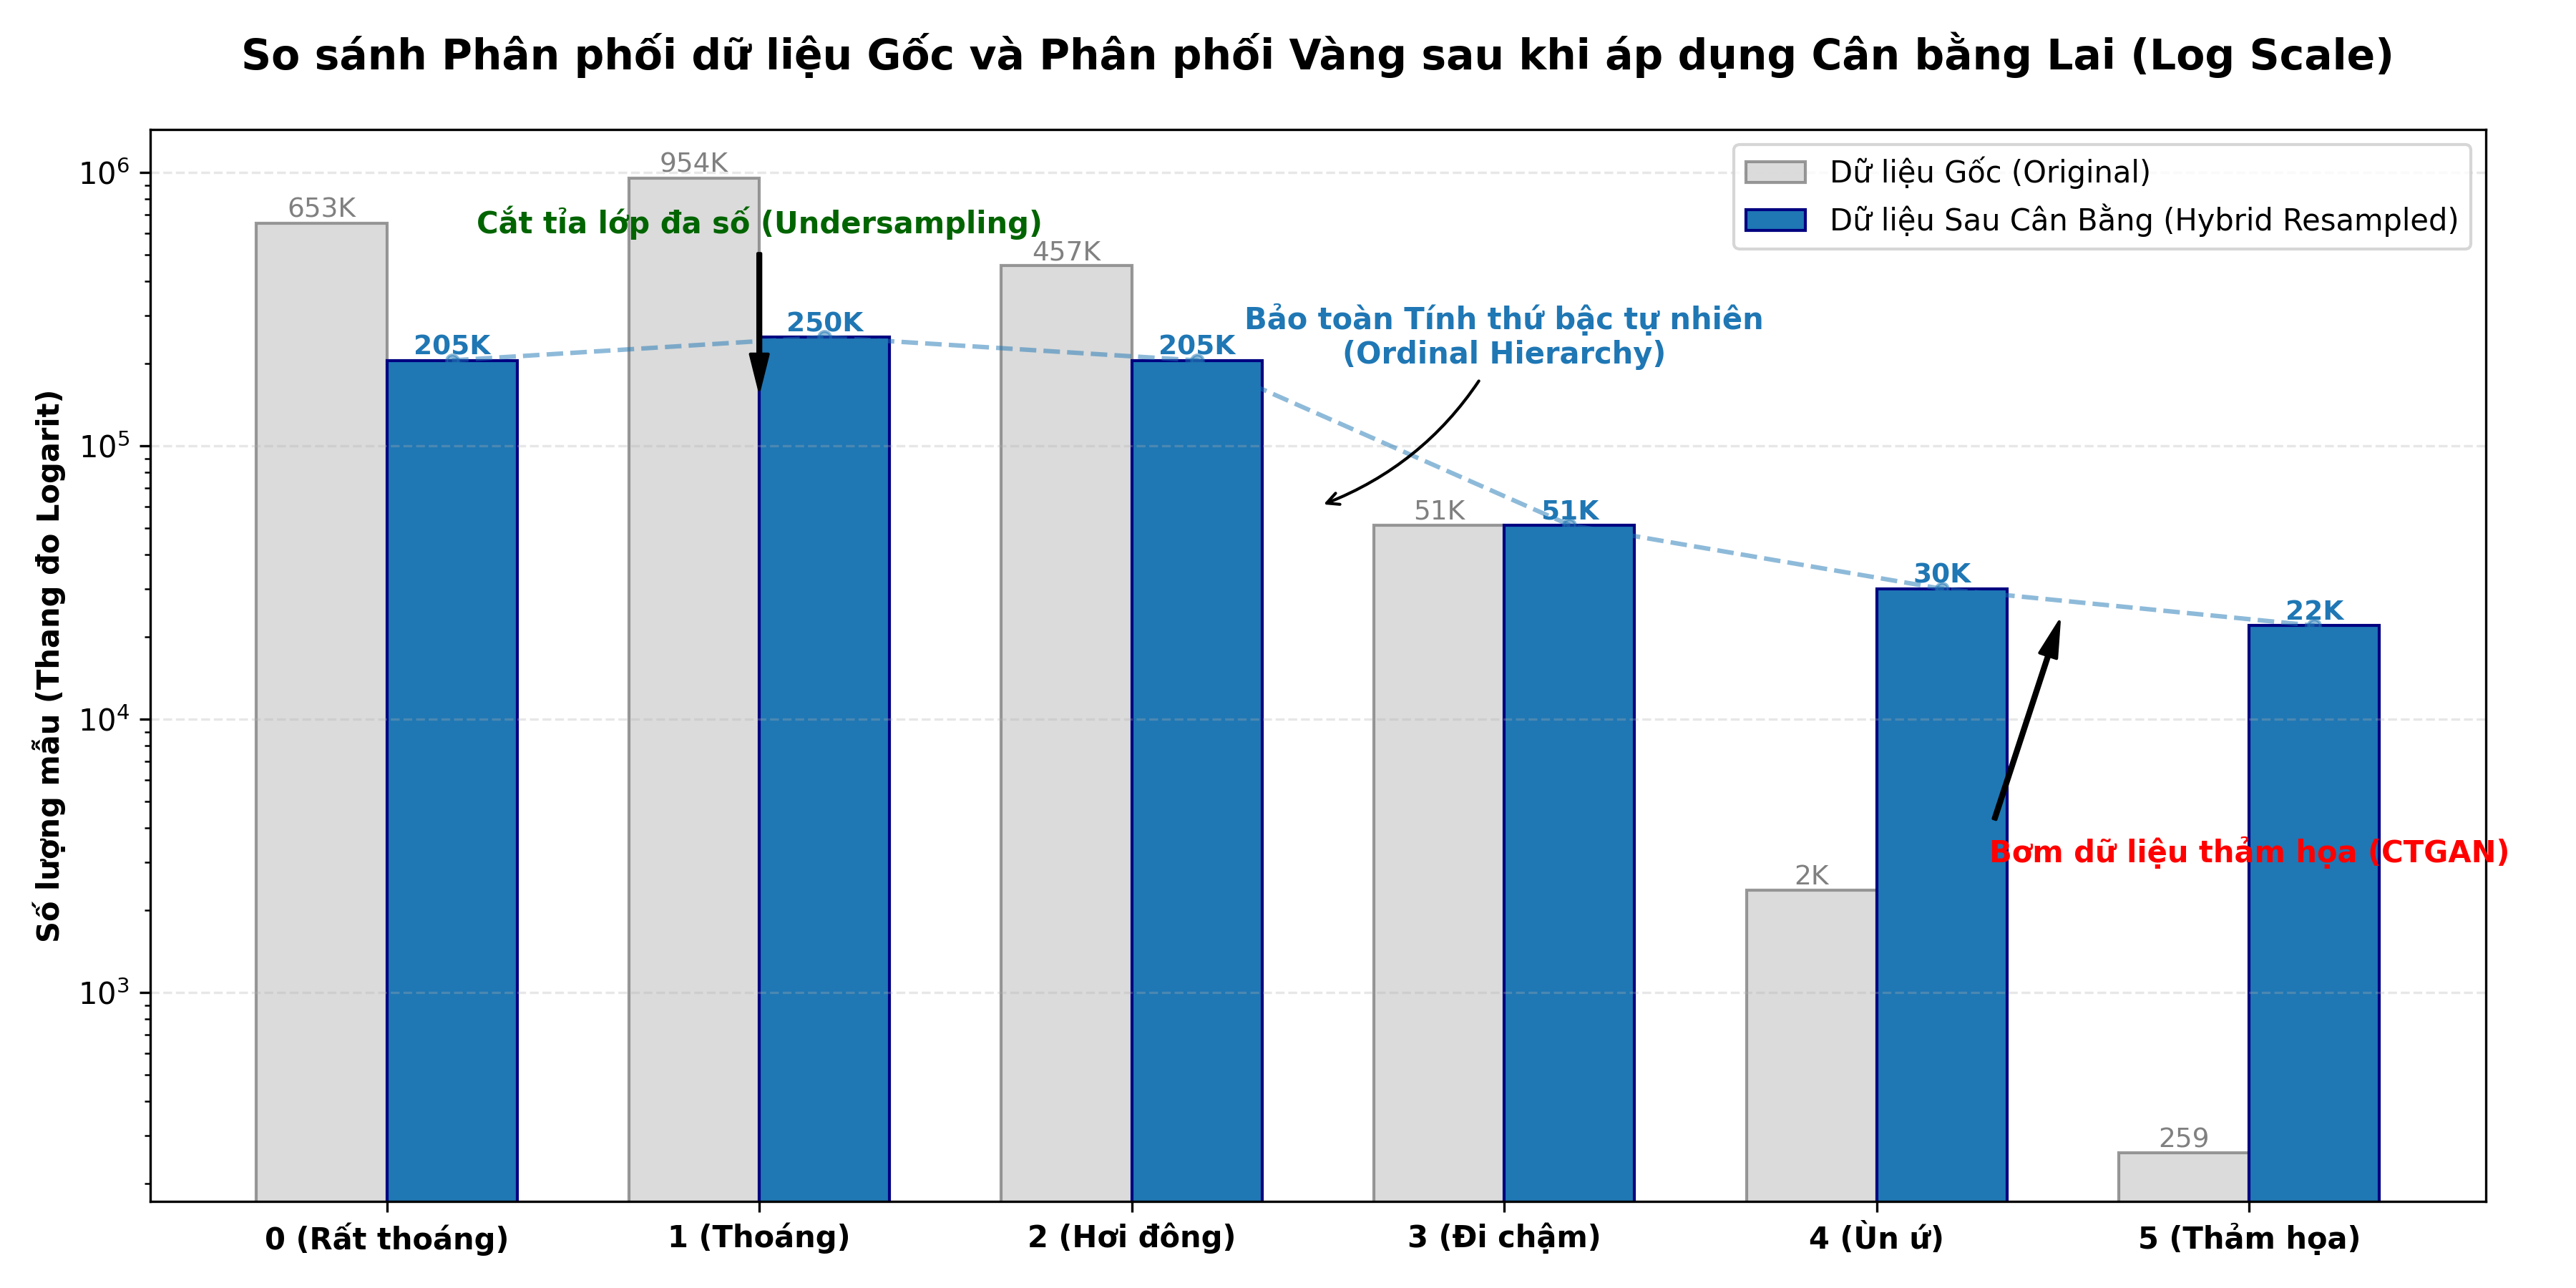
\includegraphics[width=0.8\textwidth]{Images/CH5/11a.png}
    \vspace{12pt}
    \caption{So sánh Phân phối dữ liệu Gốc và Phân phối Vàng sau khi áp dụng Cân bằng Lai}
    \label{fig:5_11}
\end{figure}

\subsubsection{Phân tích điểm yếu của phương pháp nội suy tuyến tính (SMOTE/ADASYN)}

Trong các bài toán Học máy truyền thống, để giải quyết vấn đề mất cân bằng dữ liệu, các kỹ thuật sinh mẫu nhân tạo như SMOTE (Synthetic Minority Over-sampling Technique) hoặc ADASYN thường là lựa chọn mặc định. Tuy nhiên, trong bối cảnh đồ án này, các phương pháp trên đã bị loại bỏ hoàn toàn khỏi kiến trúc hệ thống sau quá trình đánh giá rủi ro thuật toán.

\paragraph{a. Cơ chế nội suy tuyến tính và sự vi phạm Động lực học Giao thông} \mbox{} \\
Bản chất cốt lõi của SMOTE và ADASYN là tạo ra dữ liệu mới bằng phép Nội suy tuyến tính (Linear Interpolation). Thuật toán sẽ chọn ngẫu nhiên một mẫu thiểu số, tìm $k$ láng giềng gần nhất của nó (k-Nearest Neighbors) trong không gian đặc trưng n-chiều, và vẽ các đường thẳng nối giữa chúng để tạo ra các điểm dữ liệu ảo nằm dọc trên các đoạn thẳng đó.

Tuy nhiên, giao thông đô thị là một hệ thống vật lý phức tạp. Động lực học dòng xe (Traffic Flow Dynamics) bị chi phối bởi các ràng buộc phi tuyến nghiêm ngặt (Ví dụ: Mối quan hệ giữa Vận tốc - Mật độ - Lưu lượng thường được mô tả bằng các đường cong bậc hai parabol theo mô hình Greenshields, không phải đường thẳng). Việc SMOTE thực hiện nội suy một cách mù quáng (blind interpolation) cắt ngang qua không gian trạng thái phi tuyến này sẽ phá vỡ hoàn toàn các định luật vật lý cơ bản.

\paragraph{b. Hiện tượng "Trạng thái Ảo giác Phi vật lý" (Unphysical Hallucinations)} \mbox{} \\
Hậu quả trực tiếp của việc dùng SMOTE là sự xuất hiện của các điểm dữ liệu nằm ngoài "quỹ đạo vật lý" cho phép.

\textbf{Ví dụ minh họa:} Giả sử có hai mẫu kẹt xe thực tế: Điểm A (Vận tốc rất thấp, đang mưa to) và Điểm B (Vận tốc trung bình, trời tạnh ráo nhưng ngay sát ngã tư). Khi SMOTE nội suy tuyến tính giữa A và B, nó có thể vô tình sinh ra điểm C mang đặc tính lai tạp: \textbf{Mật độ xe đang kẹt cứng (đặc tính của A), nhưng vận tốc dòng xe lại vọt lên 60 km/h (đặc tính của đường vắng)}.

Trạng thái C này không bao giờ có thể tồn tại trong thực tế. Đồ án định nghĩa đây là các \textbf{"Trạng thái Ảo giác Phi vật lý" (Unphysical Hallucinated States)}.

\begin{figure}[H]
    \centering
    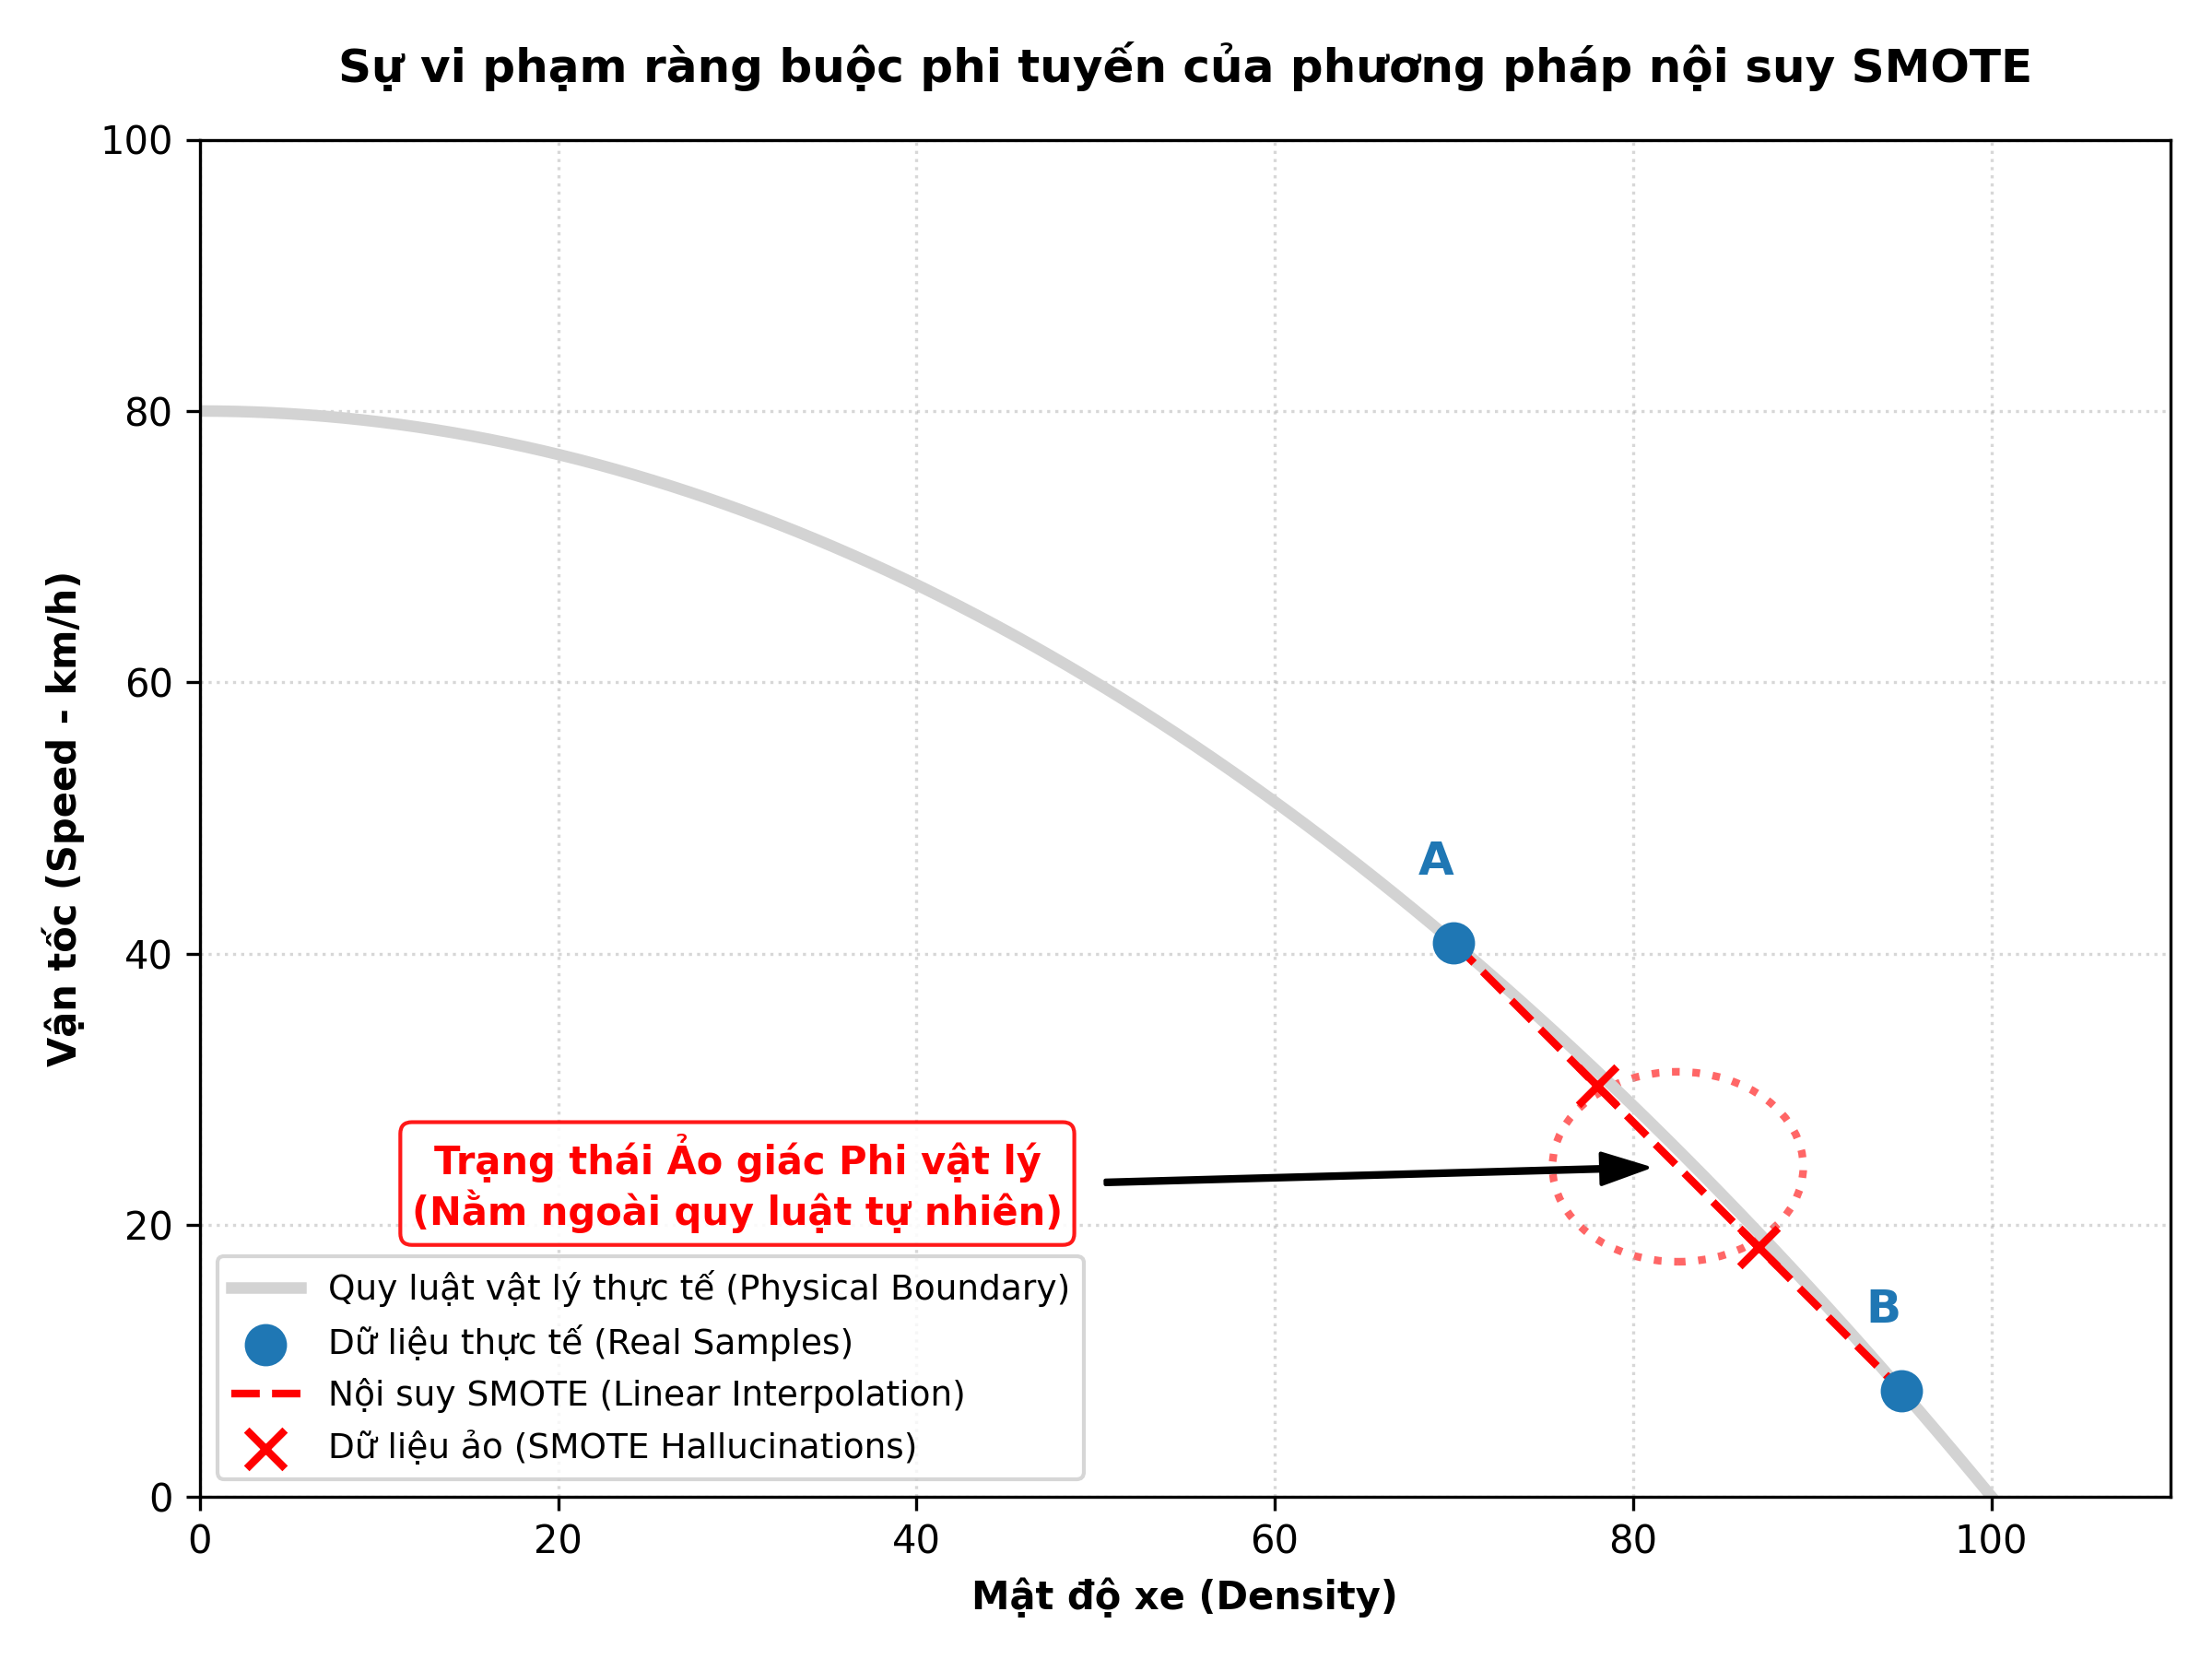
\includegraphics[width=0.8\textwidth]{Images/CH5/12.png}
    \vspace{12pt}
    \caption{Sự vi phạm ràng buộc phi tuyến của phương pháp nội suy SMOTE}
    \label{fig:5_12}
\end{figure}

\paragraph{c. Hậu quả trí mạng đối với Đặc vụ Học tăng cường (DQN Agent)} \mbox{} \\
Đối với một mô hình phân lớp thống kê đơn giản, vài điểm dữ liệu ảo giác có thể chỉ làm giảm nhẹ độ chính xác (Accuracy). Nhưng đối với mạng Double DQN – một thuật toán dựa trên việc khám phá và học luật nhân - quả từ môi trường (Markov Decision Process), hậu quả là sự sụp đổ toàn hệ thống.

Nếu các "trạng thái ảo giác" này bị tiêm vào tập dữ liệu, chúng sẽ trực tiếp đầu độc bộ nhớ kinh nghiệm (Replay Buffer). Agent sẽ học được những quy luật logic sai lệch (ví dụ: tin rằng có thể tăng tốc thoát khỏi đám kẹt xe khi mật độ đang là 100\%). Hậu quả là Hàm giá trị (Q-value) bị tính toán sai, dẫn đến việc Agent đưa ra các quyết định điều hướng hoang tưởng khi được triển khai vào môi trường thực tế.

Chính vì rủi ro "đầu độc" không gian trạng thái này, đồ án bác bỏ việc sử dụng các công cụ sinh mẫu tuyến tính truyền thống và đề xuất giải pháp mạnh mẽ hơn bằng Mô hình sinh tạo sâu (Deep Generative AI).

\subsubsection{Chiến lược Cân bằng Lai (Hybrid Resampling: Anchor-based \& Sequence-CTGAN)}

Để giải quyết triệt để rủi ro "ảo giác phi vật lý" của phương pháp nội suy tuyến tính, đồng thời khắc phục sự mất cân bằng cực hạn của dữ liệu, đồ án đề xuất và tự phát triển một chiến lược \textbf{Cân bằng Lai (Hybrid Resampling)}. Chiến lược này là sự kết hợp tinh tế giữa nghệ thuật cắt tỉa dữ liệu có kiểm soát và mô hình Trí tuệ nhân tạo tạo sinh (Generative AI), được chia làm hai nhánh xử lý song song.

\paragraph{a. Nhánh 1: Cắt tỉa thông minh dựa trên Mỏ neo (Smart Under-sampling with Anchor-based Filtering)} \mbox{} \\
Đối với nhóm dữ liệu đa số (Lớp 0, 1, 2) chiếm tới hàng trăm ngàn mẫu, việc giữ lại toàn bộ sẽ làm cạn kiệt tài nguyên tính toán và gây ra "Thiên kiến lớp đa số" (Majority Class Bias). Tuy nhiên, nếu cắt giảm ngẫu nhiên (Random Under-sampling) một cách bạo lực, hệ thống sẽ đánh mất các đặc trưng phân phối thực tế của dòng tự do.

Giải pháp được áp dụng là cơ chế \textbf{"Lọc dựa trên Mỏ neo" (Anchor-based Filtering)}.
\begin{itemize}
    \item Hệ thống lựa chọn \textbf{Lớp 3 (Kẹt xe trung bình)} làm điểm mỏ neo (Anchor) do lớp này mang tín hiệu chuyển tiếp quan trọng và có số lượng mẫu tự nhiên ở mức vừa đủ (khoảng $51.000$ cửa sổ).
    \item Dựa trên mỏ neo này, thuật toán tiến hành cắt tỉa có chọn lọc các Lớp 0, 1, và 2 xuống một ngưỡng trần (Threshold) dao động từ $200.000$ đến $250.000$ cửa sổ.
\end{itemize}
Cơ chế này đạt được mục tiêu kép: Vừa triệt tiêu khối lượng dữ liệu dư thừa (Noise reduction) giúp tăng tốc độ hội tụ của Agent DQN, vừa bảo vệ nghiêm ngặt \textbf{Tính thứ bậc tự nhiên (Ordinal Hierarchy)} của giao thông (Số lượng mẫu Lớp 1 > Lớp 0 > Lớp 2 > Lớp 3), giúp mạng Nơ-ron không bị mất phương hướng khi nhận diện bối cảnh bình thường.

\paragraph{b. Nhánh 2: Bơm máu thảm họa với Sequence-CTGAN (Over-sampling)} \mbox{} \\
Đối với nhóm thiểu số nghiêm trọng (Lớp 4 và Lớp 5), thay vì nội suy các đường thẳng vô nghĩa, đồ án ứng dụng \textbf{Mạng đối nghịch sinh tạo có điều kiện dạng bảng (Conditional Tabular GAN - CTGAN)}. Đây là một kiến trúc Deep Learning tiên tiến, bao gồm một mạng Sinh (Generator) và mạng Phân biệt (Discriminator) cạnh tranh với nhau để học được phân phối xác suất chung (Joint Distribution) đa chiều của dữ liệu thực.

Kết quả của quá trình huấn luyện đối nghịch này là hệ thống đã tổng hợp thêm thành công $30.000$ cửa sổ cho Lớp 4 và $22.000$ cửa sổ cho Lớp 5. Các điểm dữ liệu sinh ra không phải là bản sao chép, mà là các "kịch bản thảm họa" hoàn toàn mới nhưng tuân thủ tuyệt đối các ràng buộc vật lý phi tuyến của mạng lưới giao thông.

\paragraph{c. Chìa khóa thành công: Đảm bảo Tính nhất quán Chuỗi thời gian (Temporal Consistency)} \mbox{} \\
Điểm đột phá kỹ thuật đáng tự hào nhất của đồ án nằm ở cách cấu hình CTGAN. Về bản chất nguyên thủy, CTGAN được thiết kế để sinh ra các dòng dữ liệu độc lập (Single-row Tabular Data). Nếu áp dụng một cách ngây thơ vào bài toán này, nó sẽ sinh ra các timestep rời rạc, làm vỡ vụn chuỗi thời gian, khiến mạng LSTM (ở Mục 5.1.3) hoàn toàn vô dụng.

Để vượt qua rào cản này, hệ thống đã tái định dạng không gian sinh tạo: \textbf{Ép CTGAN phải sinh dữ liệu theo đơn vị Khối (Window-level Generation)}.

Mỗi mẫu dữ liệu mà CTGAN học và sinh ra không phải là một trạng thái tại thời điểm $t$, mà là một \textbf{ma trận cửa sổ trượt gồm 13 bước thời gian liên tiếp} (12 bước đầu vào + 1 bước nhãn mục tiêu). Sự điều chỉnh kiến trúc này buộc mạng Discriminator phải đánh giá sự hợp lý của toàn bộ diễn biến "sóng xung kích". Nhờ đó, dữ liệu nhân tạo được sinh ra giữ nguyên \textbf{Tính nhất quán Chuỗi thời gian (Temporal Consistency)} – vận tốc sẽ giảm dần có tính toán, độ trễ sẽ tích lũy theo từng phút, tái hiện chân thực quá trình một vụ ùn tắc giao thông dần dần lan rộng thành thảm họa vỡ trận.

\begin{figure}[H]
    \centering
    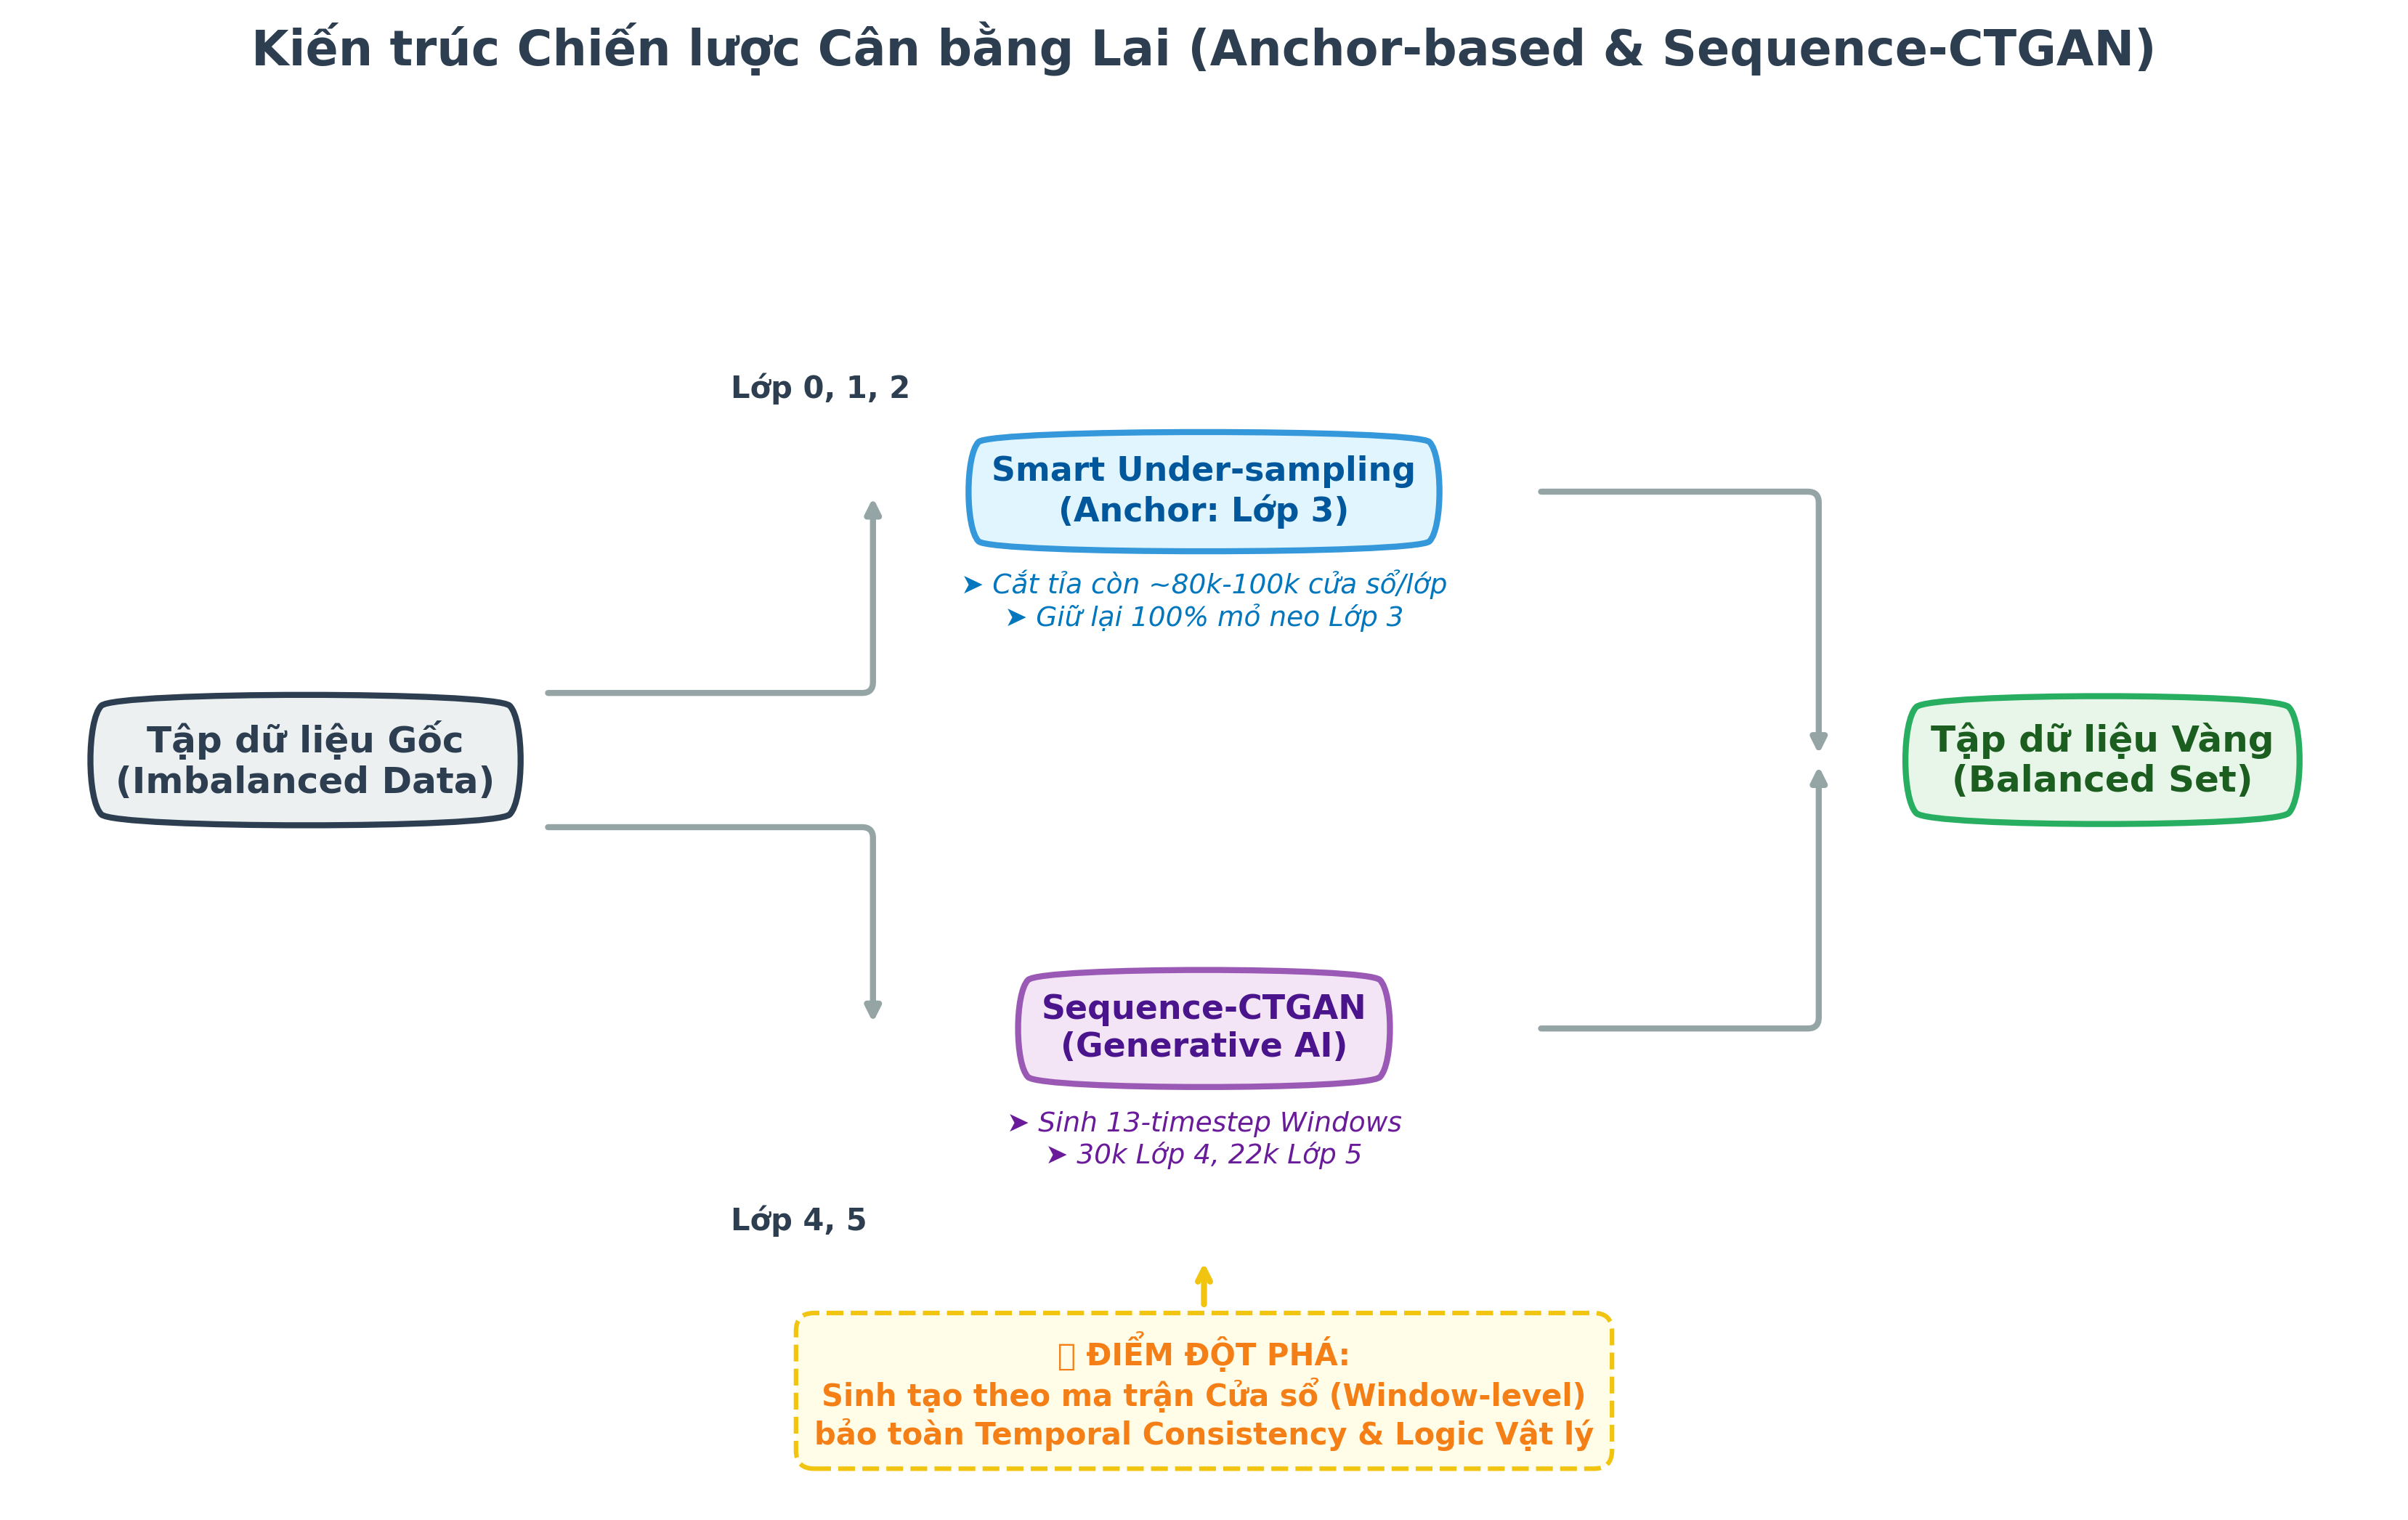
\includegraphics[width=0.8\textwidth]{Images/CH5/13.png}
    \vspace{12pt}
    \caption{Kiến trúc Chiến lược Cân bằng lai}
    \label{fig:5_13}
\end{figure}
